\documentclass[11pt,a4paper]{article}
\usepackage[utf8]{inputenc}
\usepackage[T1]{fontenc}
\usepackage{lmodern}
\usepackage{microtype}
\usepackage[a4paper,margin=1in]{geometry}
\usepackage{amsmath,amssymb}
\usepackage{booktabs,array,enumitem,tabularx}
\usepackage{graphicx}
\usepackage{xcolor}
\definecolor{accent}{HTML}{1F3A5F}
\usepackage[colorlinks=true,linkcolor=accent,citecolor=accent,urlcolor=accent]{hyperref}
\usepackage{sectsty}
\usepackage{fancyhdr}
\usepackage{setspace}
\usepackage{caption}
\captionsetup{font=small,labelfont=bf}
\setstretch{1.15}
\sectionfont{\color{accent}\large}\subsectionfont{\color{accent}\normalsize}
\pagestyle{fancy}\fancyhf{}
\lhead{\small BS Project: First Results}\rhead{\small Prince Kumar (23B3032)}
\cfoot{\thepage}\renewcommand{\headrulewidth}{0.4pt}
\setlist{itemsep=1pt,topsep=3pt}
\graphicspath{{../reports/figs/}}
\newcolumntype{L}{>{\raggedright\arraybackslash}X}
\newcommand{\bp}{\,bp}

\begin{document}

\begin{center}
{\Large\bfseries\color{accent} Limits to Arbitrage in the Indian Equity Market}\\[4pt]
{\large First Results}\\[8pt]
Prince Kumar (23B3032), BS Economics, IIT Bombay\\
Guide: Prof.\ Aditi Chaubal \quad\textbar\quad EC 495 / EC 497\\
November 2026
\end{center}
\vspace{4pt}

\section{Summary}
Since the October report I have done four things.
\begin{enumerate}
\item \textbf{Fixed the test plan in writing and froze it} before relating any mispricing measure to bans, reforms or any
other treatment. Where the plan left a detail open, I wrote the detail down with a date before running the test that
needed it. Results that I added after seeing a test are reported as exploratory.
\item \textbf{Ran every test in the plan}: four main hypotheses, corrected jointly for multiple testing, and ten secondary
ones.
\item \textbf{Estimated the no-arbitrage band} with three-regime threshold and smooth-transition models, over time and
across states, and compared it with a bottom-up cost band.
\item \textbf{Built a constraint index} for every NSE stock and quarter from frictions alone, and checked it against price
delay and earnings drift.
\end{enumerate}
The main findings: bans bind hard on trading; correction of the basis does not become one-sided in the way the model
predicts; the basis falls when a ban starts; the band is wide and asymmetric, and its edges do not move one-for-one with the
tax; entry into the F\&O segment speeds up the response of prices to market news.

\section{Two corrections to the October report}
\begin{itemize}
\item \emph{Stock lending.} The October report said that only F\&O stocks are eligible for short selling and stock lending.
Short-selling eligibility is indeed limited to F\&O stocks (SEBI circular of 5 January 2024), but the securities lending
and borrowing segment has also covered other liquid stocks since July 2013. In the daily SLB files, non-F\&O stocks account
for 6\% to 23\% of lending trades in each year from 2019. SLB trading remains thin, so the practical overnight short is
still the stock future.
\item \emph{Dates of results.} I now date quarterly results from the exchange's first dissemination time, combining its
announcements, the results filings and board-meeting dates, and map each result to the symbol the stock traded under on
that day. The filings alone often carried later re-filing times. With this and a few other checks, some counts have
changed slightly: 1,788 ban spells and 9,416 ban stock-days (October report: 1,789 and 9,414), and 8,594 results
announcements for F\&O stocks (7,910).
\end{itemize}

\section{Data added}
Daily securities-lending files (2015 to 2026), adjusted daily returns and market capitalisations for all NSE stocks, and
AMFI's monthly flows and assets of arbitrage funds (April 2018 to September 2026). The basis sample has 486,040 stock-days
for 371 stocks, 8,851 of them in a ban.

\section{Main hypotheses}
\begin{table}[h]\centering\small
\caption{The four main hypotheses (Holm correction at 5\%)}\label{tab:main}
\begin{tabularx}{\textwidth}{>{\raggedright\arraybackslash}p{3.6cm}>{\raggedright\arraybackslash}p{3.9cm}L}
\toprule
Hypothesis & Main estimate & Result \\
\midrule
Bans move trading out of futures & Futures contracts $-2.00$ log points (s.e.\ 0.11); delivery share $+0.041$ & Supported \\
Costs set the band edges & 80th percentile $+6.4$ and $+7.4$\bp\ around the 2024 and 2026 STT increases & Supported on the planned statistic; weak against placebo dates \\
Short-sale access (F\&O entry and exit) & Price delay after entry $-0.109$ (s.e.\ 0.023) & Supported through price delay; drift after bad news goes the other way \\
One-sided correction in bans & Change in reversion in a ban: upper regime $-0.089$, lower $+0.081$ & Rejected, opposite sign \\
\bottomrule
\end{tabularx}
\end{table}

\paragraph{Trading in a ban.} In a ban, futures trading falls by about 87\%, cash volume rises by about 7.5\% and more of
it is delivered. The model also predicts that every futures trade in a ban closes a long and a short, so the change in open
interest equals minus the volume. This holds almost exactly from 23 March 2020, when SEBI's measures made the clearing
corporations judge ban violations on peak intraday positions, and not before, when only end-of-day positions counted
(Figure~\ref{fig:R}).

\begin{figure}[h]\centering
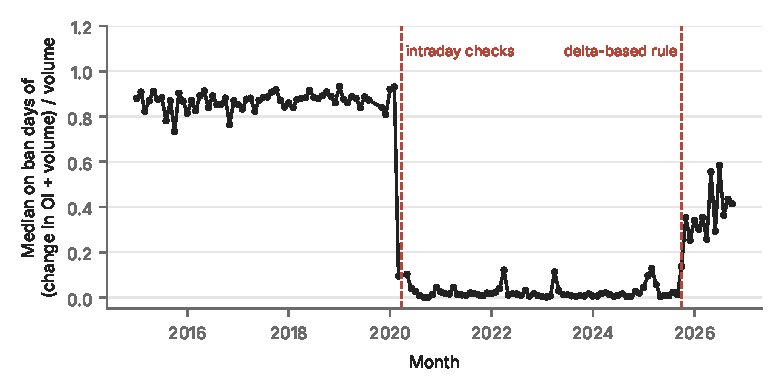
\includegraphics[width=0.72\textwidth]{fig_ban_R.pdf}
\caption{Monthly median of (change in open interest + volume) / volume on ban days. A value of zero means every trade
closed positions on both sides.}\label{fig:R}
\end{figure}

\paragraph{Correction in a ban.} The model predicts that rich futures stop being corrected in a ban, because nobody may open
new cash-and-carry positions. In the data, rich futures revert faster in a ban and cheap futures more slowly. The pattern is
concentrated in the first days of a spell and survives a correction for noise in daily prices. A reading consistent with
it, though formed after the test, is that at the start of a ban the model's second channel dominates: demand for new
futures exposure is blocked, which removes the pressure that had made futures rich.

\paragraph{Costs.} Around the 2024 and 2026 STT increases the upper part of the basis distribution rose, and the ordering of
the three increases matches the size of the cost changes. At 30 placebo dates, however, the same statistic varies by about
7\bp, because shocks common to all stocks move the whole distribution; the rise is mostly such a shift, and larger than the
cost changes.

\paragraph{F\&O entry and exit.} After a stock enters the F\&O segment its price responds much faster to market-wide news,
and after an exit somewhat more slowly. Drift after bad news becomes stronger, not weaker, after entry. Entry requires a
stock to have grown, which by itself speeds price adjustment; the leads before entry are flat, but this cannot be ruled out.

\section{Secondary results}
\paragraph{The level of the basis when a ban starts.} Against stocks that came close to 95\% but did not cross it, matched on
their utilisation path and basis, the basis falls by about 6\bp\ in the first days of a ban and recovers after about a week
(Figure~\ref{fig:level}). The fall is larger when open interest had been building fast before entry, as the model's level
result implies; the planned split (rising against falling open interest) has the predicted signs but only 30 events with
falling open interest ($p=0.08$), while a median split and a continuous measure are significant.

\begin{figure}[h]\centering
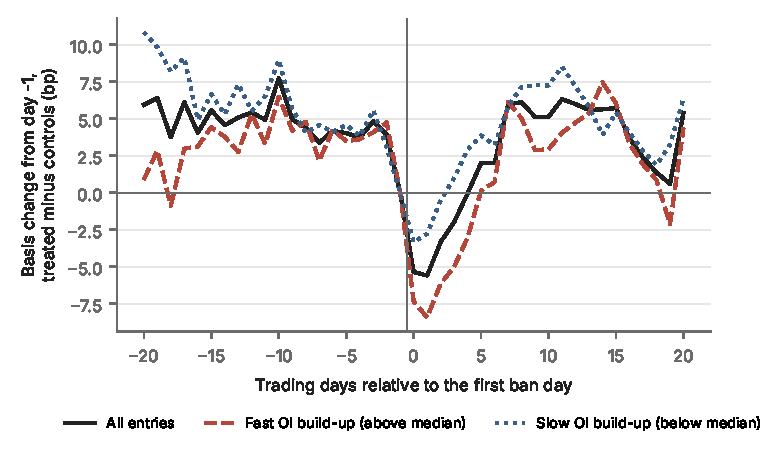
\includegraphics[width=0.75\textwidth]{fig_level_profile.pdf}
\caption{Change in the basis from the day before a ban starts, banned stocks minus matched controls.}\label{fig:level}
\end{figure}

\paragraph{The 95\% trigger.} Utilisation does not bunch below the trigger (density test $p=0.86$); it accelerates toward it.
At the trigger, futures trading drops sharply, while the basis is already lower on the day utilisation crosses 95\%. As
utilisation approaches the trigger on days without a ban, the basis is more often rich (Figure~\ref{fig:h9}). Between 80\%
and 95\%, at equal utilisation and recent basis, being in a ban does not move the basis further.

\begin{figure}[h]\centering
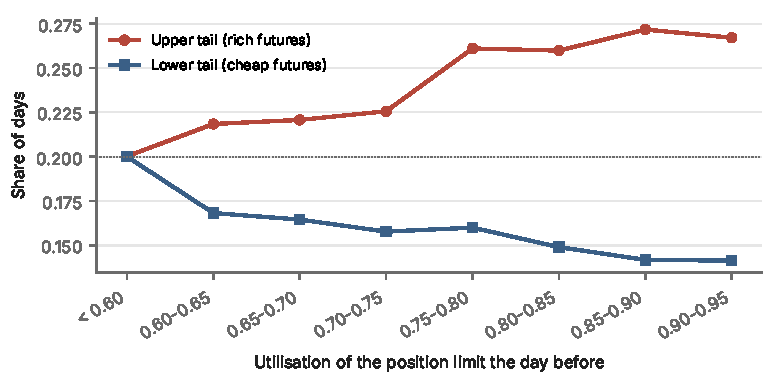
\includegraphics[width=0.72\textwidth]{fig_h9_tails.pdf}
\caption{Share of days with the basis in the stock's upper and lower tail, by utilisation the day before (days without a
ban, before October 2025; raw shares). With date effects removed the upper-tail rise remains and the lower-tail decline
disappears.}\label{fig:h9}
\end{figure}

\paragraph{Other secondary tests.} The October 2025 change in the position-limit formula moved utilisation strongly; its
effect on the basis is in the predicted direction but not significant. Bad news in bans could not be tested with useful
precision (55 events). Across stocks, higher frictions go with wider bands. Inflows into arbitrage funds are followed by a
lower upper tail of the basis, but the evidence is weak. Anomaly returns do not show the predicted asymmetry between
constrained and unconstrained stocks once returns are value-weighted.

\section{The no-arbitrage band}
I estimate three-regime threshold models of the daily change in the basis on the lagged deviation from each stock's median
(non-ban days, 473,110 observations), with a bootstrap test of linearity and bootstrap intervals for the thresholds, and
compare them with smooth-transition models.
\begin{itemize}
\item The band is about $-35$ to $+24$\bp\ around each stock's median, and linearity is clearly rejected. The threshold model
fits best; a logistic smooth-transition model, which allows different speeds below and above, fits almost as well; a
symmetric exponential one fits worse.
\item Noise in daily prices inflates the measured speed of reversion. Instrumenting the lagged deviation with its own lag
removes most of the apparent reversion inside the band and most of the difference between the two outer regimes.
\item The band is wider far from expiry; reversion is faster in the last week before expiry, slower when utilisation is high,
and faster when arbitrage-fund assets are large (in smooth-transition models with these states).
\item A new cash-and-carry round trip costs 27 to 31\bp\ (STT, stamp duty, exchange charges and brokerage), which places it in
the outer tail of the basis, while rolling an existing position costs 4 to 8\bp. This is one reason why estimated edges sit
inside the full cost band.
\end{itemize}

\begin{figure}[h]\centering
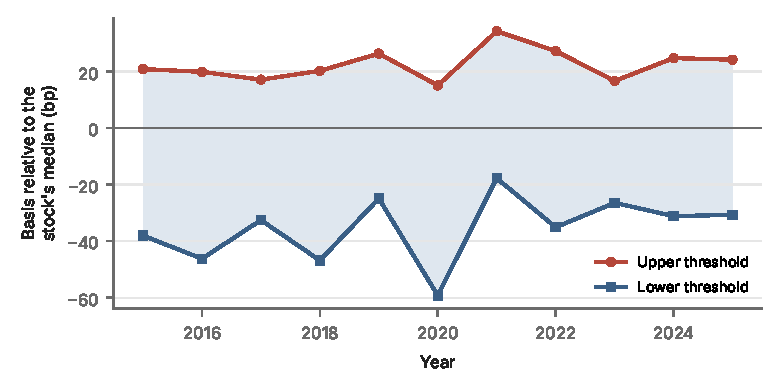
\includegraphics[width=0.72\textwidth]{fig_band_years.pdf}
\caption{Estimated band edges by year (basis relative to each stock's median).}\label{fig:band}
\end{figure}

\section{A constraint index}
For all 3,310 NSE stocks and each quarter from 2015 to 2026, the index combines five frictions: no short channel, scarcity
of stock lending, the Corwin-Schultz spread, Amihud illiquidity and idiosyncratic volatility (first principal component, 53\%
of their variance, stable loadings). More constrained stocks respond more slowly to market news the next year, also within a
stock over time and after controlling for size. Their stronger drift after bad news is a size effect: it disappears with a size
control. Within F\&O stocks a separate index that adds utilisation of the
position limit is the relevant measure for the futures-cash band.

\section{Plan from here}
\begin{enumerate}
\item Complete the thesis chapters; a full draft with all results exists, and I can share it.
\item Read the three papers I could not obtain online (Saurav, Srivastava and Agarwalla 2026; Gagnon 2018; Brennan and
Schwartz 1990) and position the ban results against the first.
\item Revisit the 2025 reform as more post-reform data arrive.
\end{enumerate}
I would value your views on two points: whether the interpretation of the one-sided-correction result (blocked new demand at
the start of a ban) should be developed into an extension of the model, and whether the smooth-transition models with
observed states should be taken further for the band chapter.

\end{document}
